\documentclass[../main.tex]{subfiles}

\begin{document}
\section{Support Vector Machines}
Support Vector Machines(SVM) is a kernel method that was very famous during the 90s. Is one of the most theoretical complete method in the machine learning world. Its theoretical guarantee are very good, and they reflect also in practice. The topic is very complex, so the goal of this chapter is to explain the most salient points.
SVM are composed by three elements
\begin{enumerate}
    \item \textbf{Subset of training data} Being a kernel method the complexity depends on the number of samples we consider. SVM works on particular subset of training samples to reduce complexity and find sparser solutions. This subset is called \textbf{support vectors}
    \item \textbf{Vector of weight $\boldsymbol{\alpha}$} This vector is used to weight the training samples subset.
    \item \textbf{Kernel} SVMs are a kernel method, so they need a similarity function(kernel) to work.
\end{enumerate}
SVM is mainly used for classification. From now on we will consider a binary classification problem. In this case, the class prediction for a new example $x_q$ is
\begin{align*}
     & f(x_q) = sign\bigg( \sum_{m \in \mathcal{S}} \alpha_m t_m k(x_q,x_m) + b \bigg) \text{, where} \numberthis \\
     & \mathcal{S} \text{ set of indices of the support vectors}                                                  \\
     & \alpha \text{ vector of weights}                                                                           \\
     & t \text{ target vector}                                                                                    \\
     & k(x_q,x_m) \text{ kernel}
\end{align*}
We can see that the solution formulation is somewhat similar to the one of the perceptron. In fact, usually SVMs are presented as their generalization. Now we will try to explain how we can derive this solution by revisiting the perceptron.
We know that the prediction for perceptron is define as
\begin{equation*}
    f(x_q) = sign(w^T \Phi(x_q)) = sign \bigg(\sum_{j=1}^M w_j \Phi_j(x_q) \bigg)
\end{equation*}
We can also recall that the various weight are updated using gradient descent as
\begin{equation*}
    w^{(k+1)} = w^{(k)} + \alpha \Phi(x_n)t_n
\end{equation*}
where the superscript indicate the iteration step. If we assume that every weight start from zero, every weight can be calculated as
\begin{equation*}
    w_j = \sum_{n=1}^N \alpha_n t_n \Phi_j(x_n)
\end{equation*}
Now we can put our new formulation of $w_j$ into the perceptron function
\begin{align*}
    f(x_q) & = sign \bigg( \sum_{j=1}^M \bigg( \sum_{n=1}^N \alpha_n t_n \Phi_j(x_n) \bigg) \Phi_j(x_q) \bigg) \\
           & = sign \bigg( \sum_{n=1}^N \alpha_n t_n (\Phi(x_n) \Phi(x_q)) \bigg) \numberthis
\end{align*}
We can observe that the only elements dependent on m are the features $\Phi_j$. We can rewrite the sum over m as a dot product between $\Phi(x_q)$ and $\Phi(x_n)$. Doing so, the sum over features as been rewritten as a sum over the samples. Furthermore, the feature appears only as dot product, so we can find a kernel representation for this function. What before was a parametric method, now is an instance-based method. Our prediction is now become a weighted average over the target value and the similarity between the input and the training data samples. What we are doing is like a weighted kNN.
Now, one can argue that this method has parameter even though it is non-parametric. Non-parametric it doesn't mean that our method doesn't have parameters, but that they are related to the samples, instead of the features, as we can see in the example above.

To obtain a SVM from the perceptron we can replace the dot product with an arbitrary kernel $k(x,x')$. A very good property of SVM is that the usage of kernels ensure a convex weight optimization problem. In practice, we can always find the global optimum.

\subsection{Learning phase}
In the learning phase of SVM we need to define three things
\begin{itemize}
    \item \textbf{Kernel} To choose a kernel we don't have a general approach, because it is highly dependent on the problem formulation
    \item \textbf{Training subset} We will see how this is a side effect of choosing the weights. In short, if a weight relative to a sample is zero, it will be excluded from the subset
    \item \textbf{Weights} The weights are calculated maximizing the margin.
\end{itemize}
Now we don't have a clue on what the margin is. Let's define it.
To better understand the concept consider the figure below. We want to find the line that separate the two classes (+) and (-). We have found two decision boundaries corresponding to the red and blue lines. Which is the better solution? One can argue that the blue solution is better because is more "centered" between the two classes. In a more formal way, the blue line have a greater distance to the nearest point comparing to the red line.
\begin{definition}[Margin]
    The margin is the minimum distance between the decision boundary hyperplane and the nearest point.
\end{definition}

\begin{center}
    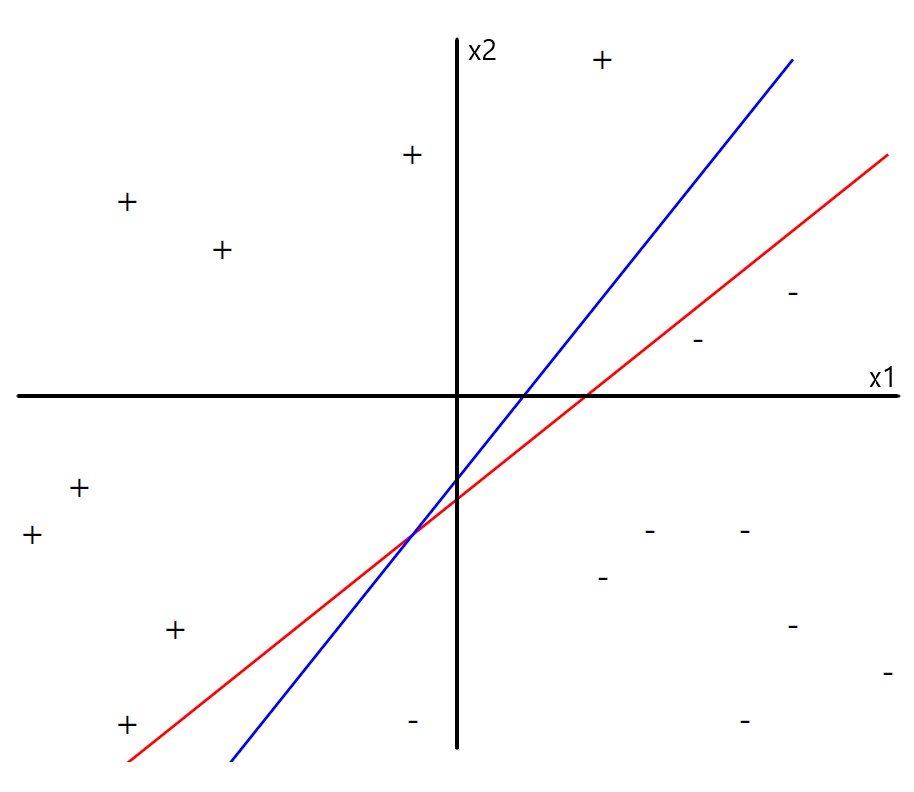
\includegraphics[width=90mm]{images/SVM_Margin.PNG} \\
    2-dimensional input space with two classes (+) and (-). \\
    Both red and blue line are linear separators of the two classes
\end{center}
In formulas we have
\begin{equation}
    margin = \underset{n}{min} (t_n (w^T \Phi(x_n) + b))
\end{equation}
As we have seen in section 1.1.1, the distance between a point and the decision boundary is expressed as $\frac{y(x_n)}{\|w\|_2}$. In our case $y(x_n)$ is simply $w^T\Phi(x_N) + b$. We can see that $\|w\|_2$ doesn't depend on $x_n$, so it can be dropped for points comparison. Furthermore, we can, for the moment, make the assumption that all the points are classified correctly by the boundary. Knowing that, we can multiply $y(x_n)$ by $t_n$, to ensure that the margin is always positive.
\newline
To find the optimal weights we need to maximize the margin.
\begin{equation*}
    w^* = \underset{w,b}{argmax} \bigg( \frac{1}{\|w\|_2} \underset{n}{min} (t_n (w^T \Phi(x_n) + b)) \bigg)
\end{equation*}
Another reason why we removed $\|w\|_2$ from the margin, is to ensure that it later reappear in $w^*$ formulation.
The direct solution computation from the formula above is very complex, because nesting a minimization inside a maximization is very computational intensive. So we need to consider an equivalent problem that is easier to be solved. Another reason why the complexity is high, it is due to the fact that an hyperplane(decision boundary) can be expressed in an infinite number of ways\footnotemark.\footnotetext{For example $3x_1+\frac{1}{2}x_2 = c$ is the same hyperplane as $6x_1+x_2 = 2c$} We can solve this by fixing the scale of the parameters. We do so by imposing the margin equal to 1. Doing so, we are sure that only one combination of $w$ will satisfy this condition. This solves also the min-max nesting, because in the new problem formulation we can drop the min computation and consider the margin as a constraint where $margin \geq 1$.

From this considerations we can formulate the new problem. First, we can eliminate the margin from $w*$.
\begin{align*}
     & w^* = max \bigg( \frac{1}{\|w\|_2} \bigg),   \\
     & \text{where } t_n (w^T \Phi(x_n) + b) \geq 1
\end{align*}
For notations purposes, we switch from a maximization problem to a minimization one. We also slightly modify it to have simpler calculi later on
\begin{equation*}
    w^* = min \bigg( \frac{1}{2} \|w\|_2^2) \bigg)
\end{equation*}
Finally the new problem is
\begin{align*}
    \textbf{Minimize} \quad   & \frac{1}{2} \|w\|_2^2                           \\
    \textbf{Subject to} \quad & t_n (w^T \Phi(x_n) + b) \geq 1, \quad \forall n
\end{align*}
\paragraph{Note - Constraint optimization basics}Suppose we have
\begin{align*}
    \textbf{Minimize} \quad   & f(w)                      \\
    \textbf{Subject to} \quad & h_i(w), \quad i=1,2,\dots
\end{align*}
Where $f(w)$ is a convex function. If $f$ and $h_i$ are linear we can use linear programming, but in our case the function to minimize is actually quadratic. In this case, we need to use quadratic programming. To solve this we use a Lagrangian formulation using the Lagrange multiplier. We will give only an intuition of the method, because the complete formulation is outside the scope of this summary. In practice, we want to transform a constrained optimization problem into an unconstrained optimization problem, where the constraints are encoded into the objective function as follow
\begin{equation}
    L(w, \lambda) = f(w) + \sum_i \lambda_i h_i(w)
\end{equation}
The $\lambda_i$s are called Lagrange multiplier and $L(w, \lambda)$ is called Lagrangian function. From the constraint theory, we know that to calculate the optimal solution, we need to find a point that satisfies
\begin{equation*}
    \nabla L(w,\lambda) = 0
\end{equation*}
We can see that now we need to find both the optimal $w$ and optimal $\lambda$. Let's see an example to better understand what's going on. Suppose we have
\begin{align*}
    \textbf{Minimize} \quad   & \frac{1}{2}(w_1^2+w_2^2) \\
    \textbf{Subject to} \quad & w_1+w_2=1
\end{align*}
The  Lagrangian function would be
\begin{equation*}
    L(w,\lambda) = \frac{1}{2}(w_1^2+w_2^2) + \lambda (w_1+w_2-1)
\end{equation*}
So we find the gradient of $L(w^*,\lambda^*) = 0$
\begin{align*}
    \nabla L(w, \lambda) = 0 \rightarrow
     &
    \begin{cases}
        \frac{\partial L}{\partial w_1} = w_1 + \lambda = 0     \\
        \frac{\partial L}{\partial w_2} = w_2 + \lambda = 0     \\
        \frac{\partial L}{\partial \lambda} = w_1 + w_2 - 1 = 0 \\
    \end{cases} \\
     &
    \begin{cases}
        w_1 = \frac{1}{2}      \\
        w_2 = \frac{1}{2}      \\
        \lambda = -\frac{1}{2} \\
    \end{cases}
\end{align*}
\begin{center}
    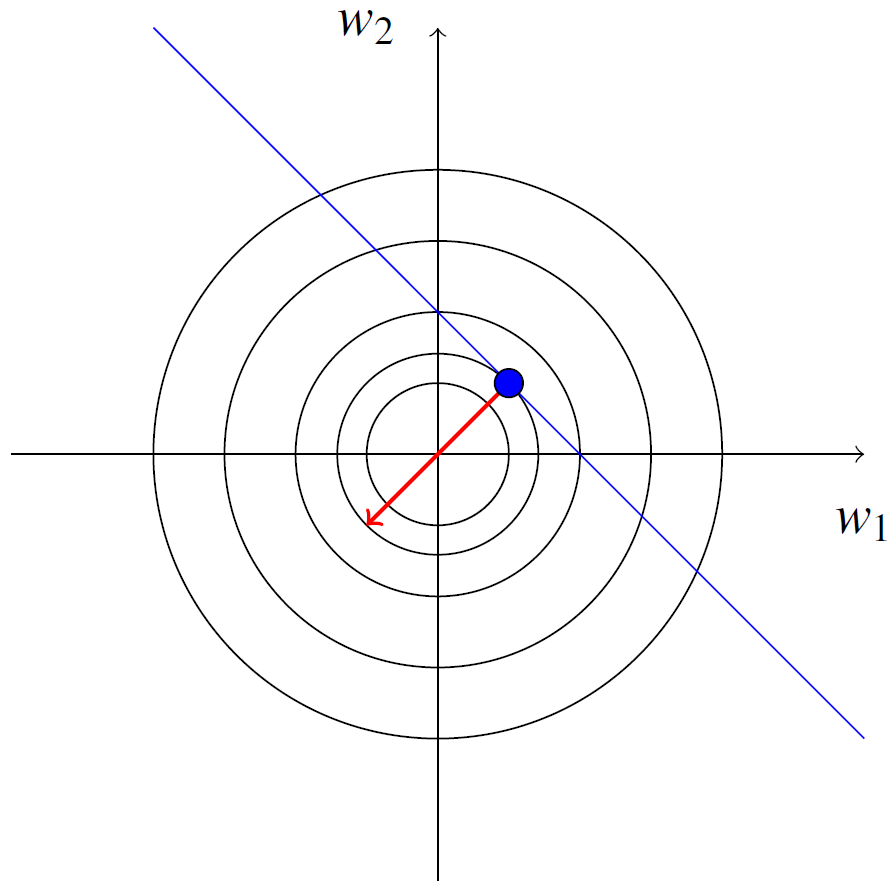
\includegraphics[width=90mm]{images/Lagrange_Multiplier.png} \\
    Black line are the isoline of our objective function. \\
    The blue line is our constraint. \\
    The red arrow is the gradient of the objective function
\end{center}
We can notice from the figure above, that the gradient of the objective function is orthogonal to the constraint. This is the same as saying that the constraint is tangent to a isoline. We know that the solution of the optimization problem must lie on the constraint. If we consider the tangent point, we can see how moving along the constraint will surely get to higher values of the objective function. This is due to the convexity of the objective function.
\newline
This is not exactly what we were looking for, because the constraint in the example was an equality and not an inequality as in our case. We need to expand our formulation to handle the inequalities. Suppose to have
\begin{align*}
    \textbf{Minimize} \quad   & f(w)                             \\
    \textbf{Subject to} \quad & g_i(w) \leq 0, \quad i=1,2,\dots \\
                              & h_i(w) = 0, \quad i=1,2,\dots
\end{align*}
We define a Lagrange multiplier $\alpha_i$ for the inequalities. To find the optimal solution we can exploit the \textbf{KKT conditions}(necessary conditions)
\begin{align*}
    \nabla L(w^*,\alpha^*,\lambda^*) & = 0    \\
    h_i(w^*)                         & = 0    \\
    g_i(w^*)                         & \leq 0 \\
    \alpha_i                         & \geq 0 \\
    \alpha_i^* g_i(w^*)              & = 0
\end{align*}
The most interesting constraint is the last one and it is called \textbf{complementarity condition}. We can have two cases
\begin{enumerate}
    \item $\alpha_i^* = 0 \land g_i(w^*) \leq 0$. If $\alpha_i^* = 0$, $g_i(w^*)$ can assume infinite different values
    \item $\alpha_i^* \geq 0 \land g_i(w^*) = 0$. If $g_i(w^*) = 0$, $\alpha_i^*$ can assume infinite different values
\end{enumerate}
Let's use the previous example to see the two cases
\begin{center}
    \begin{tabular}{cc}
        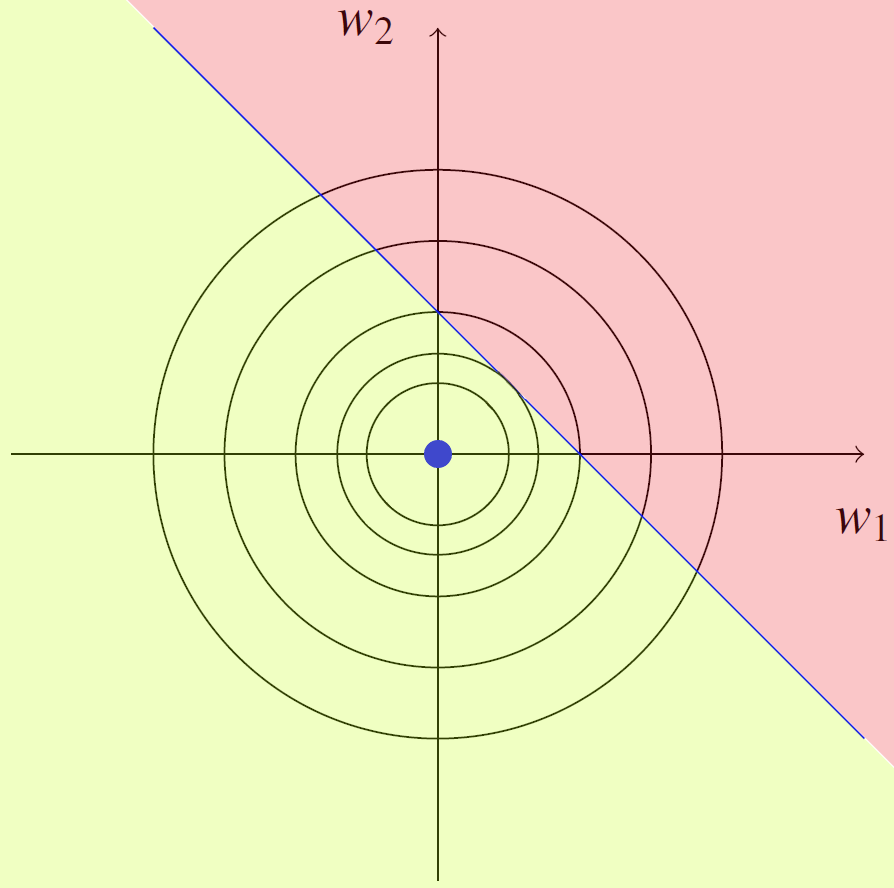
\includegraphics[width=70mm]{images/Lagrange_Multiplier_firstcase.png} & 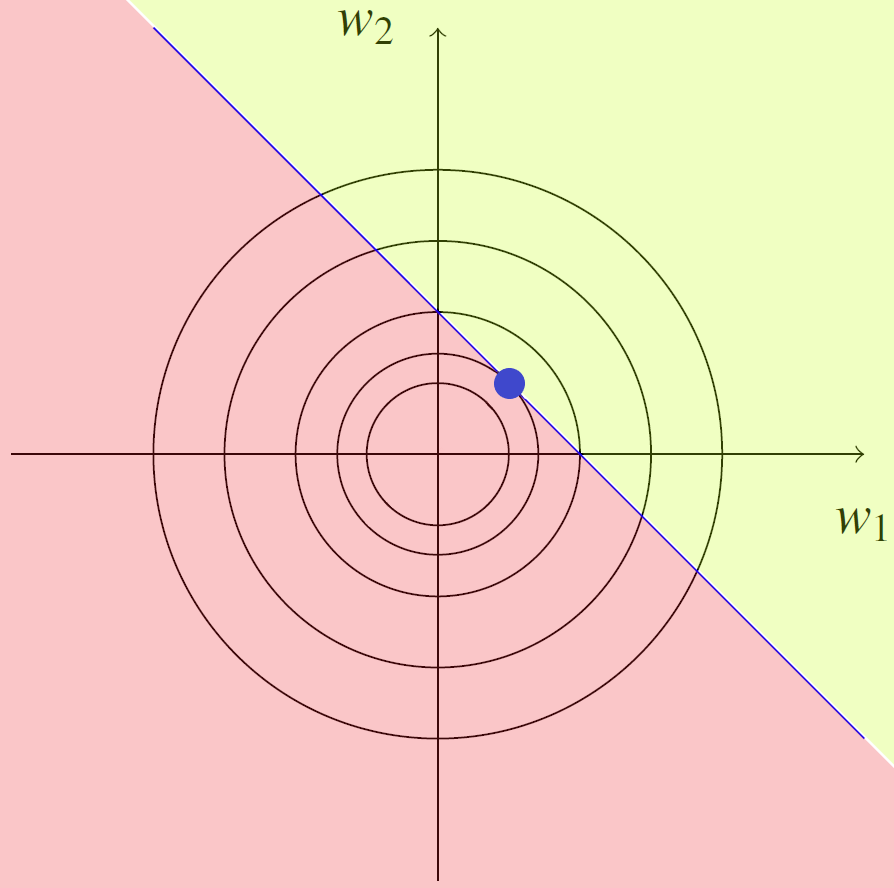
\includegraphics[width=70mm]{images/Lagrange_Multiplier_secondcase.png} \\
        (a) Case 1                                                             & (b) Case 2
    \end{tabular}
\end{center}
\newpage
In the first case we have
\begin{align*}
    \textbf{Minimize} \quad   & \frac{1}{2}(w_1^2+w_2^2)=\frac{1}{2}\|w\|_2 \\
    \textbf{Subject to} \quad & w_1+w_2 \leq 1
\end{align*}
We can see from the picture (a) above, that the solution is in the global optimum. This is due to the fact that the constraint doesn't play any role in limiting the solution. In fact, we can notice that $g(w^*) = -1$. As a consequence, we know that $\alpha = 0$, this totally make sense because the constraint is useless.

In the second case we have
\begin{align*}
    \textbf{Minimize} \quad   & \frac{1}{2}(w_1^2+w_2^2)=\frac{1}{2}\|w\|_2 \\
    \textbf{Subject to} \quad & w_1+w_2 \geq 1
\end{align*}
Here the solution is no longer in the global optimum, but lies on the constraint. In fact, we have that $g(w^*) = 0$ and $\alpha \geq 0$.

When the solution lies on the constraint, it is called active constraint. When a constraint is active its Lagrange multiplier is positive. On the other hand, if the solution is inside the region defined by the constraint, its Lagrange multiplier will be 0.
\subsection{Dual representation}
Now we have a way to solve our problem. We can observe that we have a constraint for every training sample. Now comes the very interesting part. Every sample related to a constraint with positive Lagrange multiplier will be in the support vectors set. Through weights optimization, we have found the training data subset to use for finding the solution, as we anticipated early in this section.

The optimization problem we have defined so far is called the \textbf{primal}. What we have here is still a parametric method with parameters and features.
\begin{align*}
                              & \textbf{Primal}                                 \\
    \textbf{Minimize} \quad   & \frac{1}{2} \|w\|_2^2                           \\
    \textbf{Subject to} \quad & t_n (w^T \Phi(x_n) + b) \geq 1, \quad \forall n
\end{align*}
Now our objective is to find its dual kernel representation.
Let's consider the Lagrangian function of our primal problem\footnotemark \footnotetext{Here we have a minus sign. The sign of the summation doesn't affect the solution of the Lagrangian function}
\begin{equation}
    L(w,b,\alpha) = \frac{1}{2} \|w\|_2^2 - \sum_{n=1}^N \alpha_n (t_n(w^t \Phi(x_n) + b) - 1)
\end{equation}
\newpage
As we did before, we put the gradient of $L$ equal to zero, with respect to $w$ and $b$ \footnotemark. \footnotetext{$\frac{\partial \|w\|_2^2}{\partial w} = \frac{\partial \sum_{n=1}^N w_n^2}{\partial w}\rightarrow
    \frac{\partial}{\partial w_j}\sum_{k=1}^n w_k^2=\sum_{k=1}^n \underbrace{\frac{\partial}{\partial w_j}w_k^2}_{\substack{=0, \ \text{ if } j \neq k,\\=2w_j, \ \text{ else }}}= 2w_j$. It follows that $\frac{\partial \|w\|_2^2}{\partial w}=2w$}
\newline
For $w$ we have,
\begin{align*}
    \frac{\partial L(w,b,\alpha)}{\partial w} & = \frac{1}{2} 2w - \sum_{n=1}^N \alpha_n t_n \Phi(x_n) = 0 \\
    w                                         & = \sum_{n=1}^N \alpha_n t_n \Phi(x_n)
\end{align*}
For $b$ we have,
\begin{align*}
    \frac{\partial L(w,b,\alpha)}{\partial b} & = \sum_{n=1}^N \alpha_n t_n = 0
\end{align*}
The formulation of $w$ is equal to what we have seen in the perceptron case at the beginning of this chapter. Now, we replace the new formulation of $w$ in $L(w,b,\alpha)$
\begin{align*}
                              & \textbf{Dual}                                                                                                         \\
    \textbf{Maximize} \quad   & \Tilde{L}(\alpha) = \sum_{n=1}^N \alpha_n - \frac{1}{2}\sum_{n=1}^N \sum_{m=1}^N \alpha_n \alpha_m t_n t_m k(x_n,x_m) \\
    \textbf{Subject to} \quad & \alpha_n \geq 0, \quad \text{for } n=1, \dots, N                                                                      \\
                              & \sum_{n=1}^N \alpha_n t_n = 0
\end{align*}
In this new formulation we don't have neither parameters nor features. It is an instance based formulation.
\subsection{Prediction} It's worth recalling what SVMs are doing in the input space. SVMs are linear classifier, which operates in the space defined by the features correlated to the kernel we have chosen. This highlights even more the importance of the kernel selection, because if the feature space we are defining by the kernel is not linearly separable, SVMs will fail to generate correct predictions. Another crucial point in the SVM is the optimization of the weights $\alpha$. This process is performed by applying the Lagrangian method we have seen before on the dual problem representation. Once we have $\alpha$ we can start the prediction phase.
As we said various time before, $\alpha$ defines which training samples become support vectors by giving each samples a weight. If the weight is zero, the training samples will be ignored in the boundary computation. This is a behaviour we want. Let's see an example to better visualize the problem.
\begin{center}
    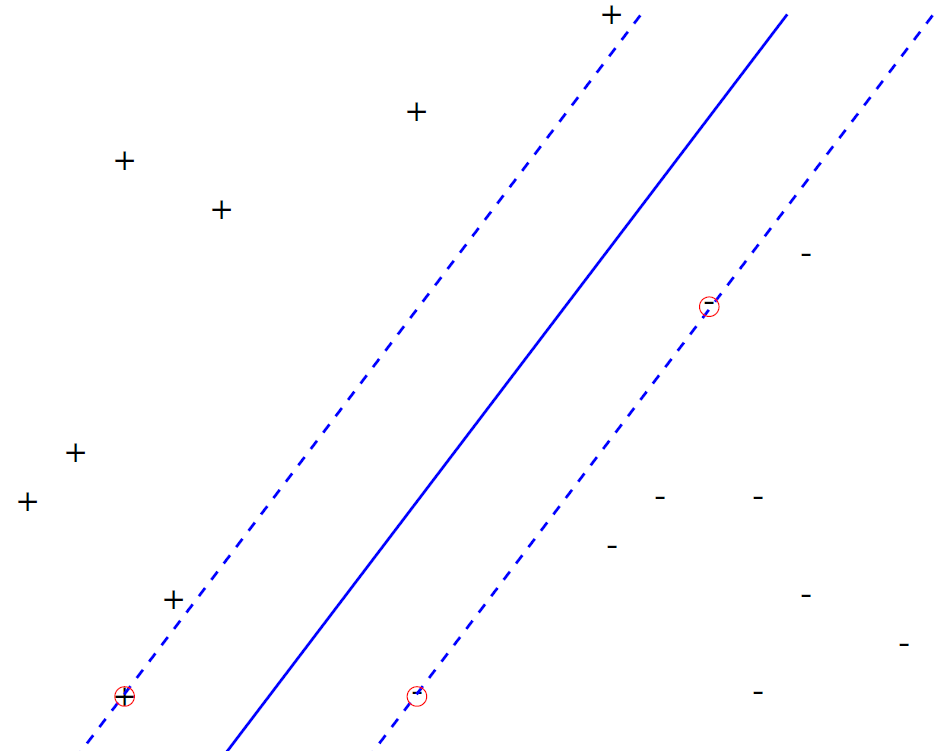
\includegraphics[width=110mm]{images/SVM_Visualization.PNG} \\
    \textit{Blue line: Decision boundary, Dashed lines: Margin, Red circles: Support vectors}
\end{center}
In the figure above we can see an important result. All the samples that don't lie on the margin are not contributing to the boundary. So all the support vector must lie on the margin. Suppose to delete a (+) sample on the top left corner. Should the boundary be changed? No, because that point doesn't affect the separation between the two classes. In practice, every samples is interpreted as a constraint. If the region they define includes the solution, the constraint is not active, and so the sample can be discarded. This is what we meant before with sparser input space. We are keeping only the samples which can contribute the most to the boundary, all the others are discarded. The ratio between the support vectors number and the number of training samples can give us some information about the performance of the SVM. The less support vectors we have the better. For example, if all the samples are also support vectors the SVM is strongly overfitting. The sparsity gives SVMs more robustness to noise and outliers, because they will be ignored.
\newline
The classification of new points is performed as
\begin{equation}
    y(x) = sign \bigg( \sum_{n=1}^N \alpha_n t_n k(x, x_n) +b \bigg)
\end{equation}
This is very similar to the perceptron case. Be aware, that we don't have a fast way to find the optimal value for $b$. We can estimate it with
\begin{equation*}
    b = \frac{1}{N_\mathcal{S}} \sum_{n \in \mathcal{S}} \bigg( t_n - \sum_{m \in \mathcal{S}} \alpha_m t_m k(x,x_m) \bigg)
\end{equation*}

Sadly, as for every method we have seen so far, the curse of dimensionality hits also the SVMs. When the number of dimensions increases, the percentage of support vectors increases too. This leads to poor generalization and to some scalability issue.
We have seen how we are able to construct bounds about the loss function of our models. For SVMs exists a very handy way to construct such bound. It's called \textbf{Leave-One-Out Bound}.
As for classic LOO, we use N-1 samples for the training phase and one sample for validation. We repeat this operation N times. We have already observed how eliminating a sample from the training set, which is not a support vector, doesn't change the solution. In this case we will not misclassify any point. In the worst case, when we "leave out" a support vector, we can misclassify a point. The loss function will be upper bounded by the probability of misclassify a point, which in our case is \footnotemark \footnotetext{$|\mathcal{S}|$ is the number of support vectors}
\begin{equation}
    L_h \leq \frac{E[|\mathcal{S}|]}{N}
\end{equation}
This bound have several computational advantages. It's like performing LOO, but without the need to train at each iteration the model, because we already know for which samples we will have a potential loss. This eliminates the major problem of LOO, but keeps the fact that is the less biased way to perform cross-validation.

\paragraph{Note - Solution technique} We have seen previously how we can solve the quadratic problem of finding the weights $\alpha$. There are more efficient way to calculate the weights. For example \textbf{SMO (Sequential Minimal Optimization)}.
Instead of calculating all the weights at the same time, we can find them in couples\footnotemark. \footnotetext{Note that if we calculate one $\alpha_i$ at the time we would violate the constraints}We can apply the following iteratively until convergence,
\begin{enumerate}
    \item Find example $x_i$ that violates KKT conditions
    \item Select second example $x_j$ heuristically
    \item Jointly optimize $\alpha_i$ and $\alpha_j$
\end{enumerate}

\subsection{Noisy data}
So far we have assumed that the data are always linearly separable. This assumption was encoded in the fact that the margin was always greater than one. Now we want to allow some samples to have a margin smaller than one, in some cases even negative. Obviously we want to minimize this behaviour, giving this points a penalization. At the same time we will relax our assumption in order to handle noisy data. The penalization is given by the \textbf{slack variables} $\xi_i$. Now we have to reformulate our primal problem to include the slack variables.
\newpage
\begin{align*}
                              & \textbf{Primal}                                         \\
    \textbf{Minimize} \quad   & \frac{1}{2} \|w\|_2^2 + C\sum_i \xi_i                   \\
    \textbf{Subject to} \quad & t_i (w^T \Phi(x_i) + b) \geq 1 - \xi_i, \quad \forall i \\
                              & \xi_i \geq 0, \quad \forall i
\end{align*}
In practice $\xi_i$ shift the margin relative to a sample $x_i$ in order to respect the constraint. But $\xi_i$ also appears in the minimization formula, in order to limit the exploitation of the margin shift. The term $C$ is a coefficient that influences how much the slack variables will penalize the objective function. If we put $C$ close to zero, we are probably making a lot of mistake, because the misclassification are not penalized. This will produce simpler models with a lot of bias and little variance. Practically we are underfitting. If $C$ tends to infinity, we are not allowed to violate the constraints. The risk is that no solution can be found, because the problem is not linearly separable. In practice, we can control the bias-variance tradeoff by manipulating this coefficient. We can find the value of $C$ with cross-validation.
As we did before we can find the dual representation
\begin{align*}
                              & \textbf{Dual}                                                                                                         \\
    \textbf{Maximize} \quad   & \Tilde{L}(\alpha) = \sum_{n=1}^N \alpha_n - \frac{1}{2}\sum_{n=1}^N \sum_{m=1}^N \alpha_n \alpha_m t_n t_m k(x_n,x_m) \\
    \textbf{Subject to} \quad & 0 \leq \alpha_n \leq C, \quad \text{for } n=1, \dots, N                                                               \\
                              & \sum_{n=1}^N \alpha_n t_n = 0
\end{align*}
We can see how $C$ has become the upper bound of $\alpha_n$. Based on the value of $\alpha_n$ we can have three cases
\begin{itemize}
    \item $\alpha_n = 0$ The point associated to $\alpha_n$ is not a support vector
    \item $0 < \alpha_n < C$ The point lies on the margin($\xi_i = 0$)
    \item $\alpha_n = C$ the point lies inside the margin, and it can be either correctly classified($0 < \xi_i \leq 1$) or misclassified($\xi_i > 1$)\footnotemark. \footnotetext{Remember that the distance between the boundary and the margin is always 1. We know that $\xi_i$ represents how much we shift the margin only for the sample $i$. If we shift it less than one, we are still correctly classifying the sample. Otherwise we are going over the boundary, and so the sample will be classified wrongly}
\end{itemize}
\begin{center}
    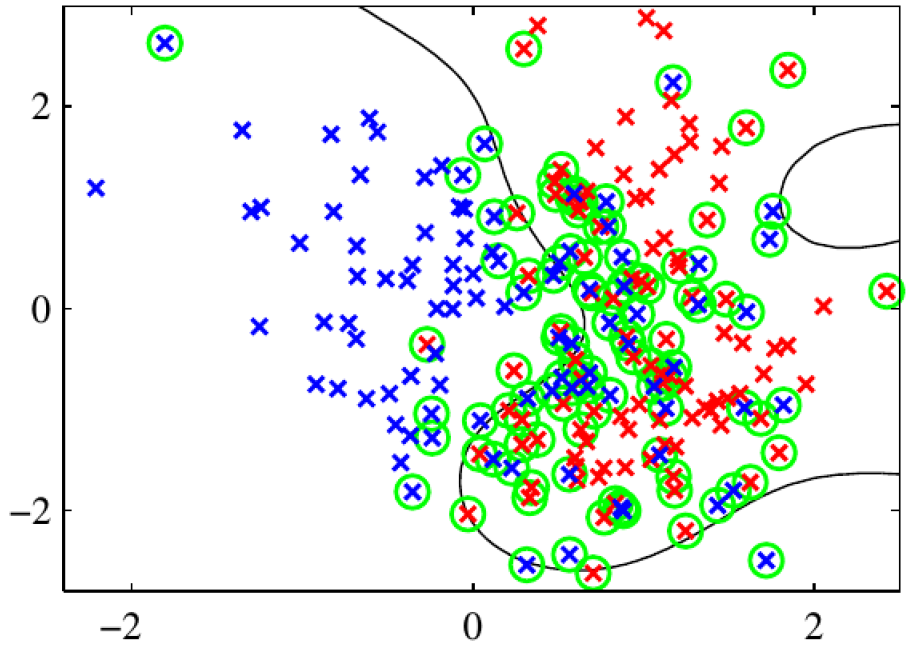
\includegraphics[width=100mm]{images/SVM_Noisy.PNG} \\
    \textit{Non linear classification problem with noisy data. Green circles: Support vectors}\\
\end{center}
In the figure above we can see an example of non-linearly separable problem. We can notice that the two classes are pretty shuffled together. This may be due to a poor kernel choice. This is also reflected in the high ratio of support vectors.
\paragraph{Note - SVM uses} So far, we have seen the SVMs applied to classification problems. We can also use them for
\begin{itemize}
    \item Regression
    \item Ranking
    \item Feature selection
    \item Clustering
    \item Semi-supervised learning
\end{itemize}

\newpage

\end{document}
